% SPDX-License-Identifier: CC-BY-4.0
\documentclass[11pt,reqno]{amsart}

\usepackage[margin=1.0in]{geometry}
\usepackage{amsmath,amssymb,amsthm,mathtools}
\usepackage{booktabs}
\usepackage{graphicx}
\usepackage{xcolor}
\usepackage{enumitem}
\usepackage{microtype}
\usepackage{tabularx}
\usepackage{hyperref}

\hypersetup{
  colorlinks=true,
  linkcolor=blue!65!black,
  citecolor=teal!70!black,
  urlcolor=blue!70!black,
  pdftitle={Thin Vieta Reflection Groups, Apollonian-Octahedral Reciprocity Obstructions, Integer-Superharmonic Sandpile Envelopes, and Markov-Hurwitz Geodesic Spectra},
  pdfauthor={Alexander Stephen Donahue}
}

\theoremstyle{plain}
\newtheorem{theorem}{Theorem}[section]
\newtheorem{proposition}[theorem]{Proposition}
\newtheorem{lemma}[theorem]{Lemma}
\newtheorem{corollary}[theorem]{Corollary}
\theoremstyle{definition}
\newtheorem{definition}[theorem]{Definition}
\newtheorem{remark}[theorem]{Remark}

\newcommand{\ZZ}{\mathbb{Z}}
\newcommand{\NN}{\mathbb{N}}
\newcommand{\QQ}{\mathbb{Q}}
\newcommand{\RR}{\mathbb{R}}
\newcommand{\SL}{\mathrm{SL}}
\newcommand{\leg}[2]{\left(\frac{#1}{#2}\right)}
\newcommand{\code}[1]{\texttt{\detokenize{#1}}}
\emergencystretch=2em
\raggedbottom

\title[Vieta Reflection Groups, Sandpile Rigidity, and Markov Spectra]{Thin Vieta Reflection Groups, Apollonian--Octahedral Reciprocity Obstructions, Integer-Superharmonic Sandpile Envelopes, and Markov--Hurwitz Geodesic Spectra: A Zero-Mathlib Six-Kernel Formalization}

\author{Alexander Stephen Donahue}
\address{Independent Researcher, Spokane, WA, USA}
\email{0\_0@0thernes.art}
\urladdr{https://0thernes.art}
\thanks{ORCID: \href{https://orcid.org/0009-0006-8168-9648}{0009-0006-8168-9648}. Archive ID: \code{0TH-2026-018}. Repository: \url{https://github.com/0thernes/apollonian-sandpile-markov}. Code licensed Apache-2.0; prose, figures, and data licensed CC-BY-4.0.}

\date{November 26, 2026}

\subjclass[2020]{Primary 11E12, 11D25, 05C50, 13F60; Secondary 11A15, 52C26, 14T10, 68V20}
\keywords{Apollonian circle packings, quadratic reciprocity, octahedral packings, Abelian sandpile, integer superharmonic functions, triangular lattice, tropical curves, Markov numbers, cluster algebras, Markov--Hurwitz equations, Lean 4 formalization}

\begin{document}

\begin{abstract}
Quadratic Vieta involutions on indefinite integral forms govern three seemingly disparate frontiers of modern mathematics: thin Lorentzian reflection groups in sphere packings, integer-superharmonic scaling envelopes of Abelian sandpiles, and the $\SL_2(\ZZ)$ Fricke--Markov geodesic spectrum. We present a unified, fully machine-checked, zero-Mathlib Lean~4.35.0 formalization of fifteen headline theorems (\code{T1a}--\code{T3e}), accompanied by constructive non-vacuity witnesses, adversarial counterexamples, independent Rust, ISO~C11 (ASan/UBSan and fuzzing), and Python/Hypothesis mutation oracles, and replay across six independent formal type-checking kernels strictly within the three standard axioms \code{propext}, \code{Classical.choice}, and \code{Quot.sound}.

Across the three pillars, our principal contributions are:
\begin{enumerate}[leftmargin=1.8em, itemsep=2pt]
\item \textbf{Pillar I (Thin Reflection Groups):} A self-contained zero-Mathlib Eisenstein~(1844) proof of Gauss Quadratic Reciprocity and Jacobi supplementary laws (\code{T1b}), powering a zero-GCD-exception parabolic Dehn-twist CRT formal proof of the Haag--Kertzer--Rickards--Stange (\emph{Annals of Mathematics}, 2024) global square obstruction on Apollonian packings (\code{T1c}), an exact generalized octahedral $\QQ(\sqrt{-2})$ mod-8 and Jacobi obstruction (\code{T1d}), and the sharp Soddy integrality dichotomy $(d-1)\mid 2 \iff d \in \{2,3\}$ (\code{T1e}).
\item \textbf{Pillar II (Sandpiles \& Tropical Curves):} Universal Abelian sandpile confluence and Discrete Least Action (\code{T2a}), exact $2\times 2$ ($192$) and $3\times 3$ ($100{,}352$) Matrix--Tree determinants via integer Kronecker block-diagonalization with explicit Dhar identity traces (\code{T2b}), Levine--Pegden--Smart $\ZZ^2$ superharmonic rigidity (\code{T2c}), an \textbf{original Triangular Lattice $\mathbb{A}_2$ Even-Laplacian Rigidity Theorem} (\code{T2d}) proving that every periodic integer superharmonic envelope on $\mathbb{A}_2$ has \emph{even} constant Laplacian $K \equiv 0 \pmod{2}$---universally obstructing the maximal stable sea $K=5$ while realizing $K \in \{2,4\}$---and universal Kalinin--Shkolnikov tropical balancing (\code{T2e}).
\item \textbf{Pillar III (Markov--Hurwitz \& Cluster Spectra):} Universal $\SL_2(\ZZ)$ Fricke--Cohn trace correspondence (\code{T3a}), pairwise coprimality, odd-prime $p \equiv 1 \pmod 4$ obstruction, and an \textbf{Exact Mod-32 Theorem} (\code{T3b}) proving every even Markov number satisfies $m \equiv 2 \pmod{32}$ (sharp modulo $64$ at $2$ and $34$), universal Hensel lifting uniqueness of $\sqrt{-1} \pmod{p^k}$ (\code{T3c}), symbolic 3-variable Fomin--Zelevinsky cluster-algebra Laurent integrality and positivity through five mutations including two consecutive non-monomial polynomial cancellations (\code{T3d}), and the complete Markov--Hurwitz $n=4$ classification via well-founded Vieta descent (\code{T3e}).
\end{enumerate}
Throughout, we maintain strict epistemic boundaries: all fifteen theorems are kernel-checked unconditionally, whereas the overarching open conjectures (full Apollonian local-global classification, continuous sandpile scaling limit \code{STAT-058}, and general-composite Markov Uniqueness \code{NT-083}) remain explicitly open.
\end{abstract}

\maketitle

\section{Introduction and the Unified Vieta-Reflection Architecture}
\label{sec:intro}

Three celebrated areas of contemporary arithmetic geometry, discrete potential theory, and algebraic combinatorics share a single algebraic engine: \emph{quadratic Vieta involutions} acting on integral lattices. Given a quadratic relation $a x_i^2 - L_i(x_{-i}) x_i + R_i(x_{-i}) = 0$ with $a=1$, flipping a root produces the involutive reflection
\begin{equation}
  x_i \longmapsto L_i(x_{-i}) - x_i,
\end{equation}
which generates an infinite discrete group of integer symmetries.
\begin{itemize}[leftmargin=1.6em]
  \item In \textbf{Pillar I (Thin Lorentzian Reflection Groups)}, the Descartes quadratic form $Q_{\mathrm{Desc}}(q) = (\sum q_i)^2 - 2\sum q_i^2$ generates the Apollonian reflection group via $b_i \mapsto 2\sum_{j\neq i} b_j - b_i$~\cite{glmw2003,bf2011,fs2011}. Recently, Haag, Kertzer, Rickards, and Stange~\cite{hkrs2024} disproved the Apollonian Local-Global Conjecture by discovering global quadratic reciprocity obstructions invisible to every congruence modulo~$24$. Analogous thin reflection groups govern generalized octahedral $\QQ(\sqrt{-2})$ packings~\cite{stange2018,kn2019} and $d$-dimensional Soddy sphere packings~\cite{lmw2002}.
  \item In \textbf{Pillar II (Abelian Sandpiles and Tropical Geometry)}, Dhar's Abelian sandpile~\cite{dhar1990} relaxes integer configurations by firing discrete Laplacian stencils $\Delta u = \sum_{e}(u(x+e)-u(x))$. Levine, Pegden, and Smart~\cite{lps2016,lps2017} revealed that the scaling limit of the $\ZZ^2$ sandpile identity is governed by \emph{Apollonian circle packings of integer superharmonic matrices} linked to the quadratic growth of the odometer, while Kalinin and Shkolnikov~\cite{ks2016,kalinin2018} showed that point perturbations on maximal seas relax into balanced piecewise-linear tropical curves.
  \item In \textbf{Pillar III (Markov--Hurwitz and Cluster Spectra)}, the Markov cubic $x^2 + y^2 + z^2 = 3xyz$ generates the Cohn $\SL_2(\ZZ)$ binary tree~\cite{cohn1955,aigner2013} through the Vieta involution $z \mapsto 3xy - z$, coincides with cluster mutations on the $2$-arrow cyclic Markov quiver~\cite{fz2002,ls2015}, and generalizes to the Markov--Hurwitz equations $\sum_{i=1}^n x_i^2 = a \prod_{i=1}^n x_i$~\cite{baragar1993}.
\end{itemize}

Rather than leaving these three themes in informal prose or fragmented computer scripts, we build a single, self-contained, zero-Mathlib Lean~4.35.0 formalization~\cite{moura2021} comprising 18 audited declarations (\code{T1a}--\code{T3e}, master conjunction, constructive non-vacuity, and sharp adversarial refutations), replayed independently across six formal type-checking kernels (including \code{lean4lean}~\cite{carneiro2024}, \code{nanoda_bin}, \code{con-leche}, and \code{con-ron}) and cross-verified bit-for-bit against independent zero-dependency Rust, ISO~C11 (ASan/UBSan + fuzz), and Python/Hypothesis/mutation oracles. Table~\ref{tab:master-map} summarizes all fifteen kernel-checked theorems and their exact epistemic boundaries.

\begin{table}[t]
\centering
\caption{Master map of all 15 kernel-checked theorems (\code{T1a}--\code{T3e}), Lean~4.35.0 module locations, independent computational oracles, and epistemic boundaries.}
\label{tab:master-map}
\footnotesize
\renewcommand{\arraystretch}{1.15}
\begin{tabularx}{\textwidth}{@{}llXll@{}}
\toprule
\textbf{ID} & \textbf{Lean Module} & \textbf{Machine-Checked Theorem Content (Zero \code{sorry})} & \textbf{Oracle} & \textbf{Scope} \\
\midrule
\code{T1a} & \code{ApollonianReciprocity} & Descartes involutions, Gaussian norm $(a+b)(a+c)=a^2+k^2$, BQF & Rust/Py/C & Universal \\
\code{T1b} & \code{JacobiReciprocity} & Zero-Mathlib Jacobi symbol, Eisenstein~(1844) QR, $\leg{-1}{n}$, $\leg{2}{n}$ & Rust/Py/C & Universal \\
\code{T1c} & \code{ApollonianReciprocity} & Zero-GCD Dehn-twist CRT proof of HKRS~\cite{hkrs2024} square obstruction & Rust/Py/C & Exact 3+1 \\
\code{T1d} & \code{ApollonianReciprocity} & Octahedral $\QQ(\sqrt{-2})$ 8 reflections, mod-8 \& Jacobi obstruction & Rust/Py & Exact 1+1 \\
\code{T1e} & \code{ApollonianReciprocity} & Soddy dichotomy $(d-1)\mid 2 \iff d\in\{2,3\}$ + 3D square hit $25=5^2$ & Rust/Py & Universal \\
\midrule
\code{T2a} & \code{SandpileTropical} & Abelian commutativity, Least Action, Church--Rosser confluence & Rust/Py & All graphs \\
\code{T2b} & \code{SandpileTropical} & Exact Matrix--Tree $\det=192, 100{,}352$ + $2\times 2, 3\times 3$ Dhar traces & Rust/Py/C & Exact grids \\
\code{T2c} & \code{SandpileTropical} & LPS $\ZZ^2$ torus Green's id, isotropic $K=3$ obstruction, $K=2,3$ & Rust/Py & Universal \\
\code{T2d} & \code{SandpileTropical} & \textbf{Original $\mathbb{A}_2$ Even-Laplacian Rigidity:} $K\equiv 0\ (2)\Rightarrow K=5$ impossible & Rust/Py/C & Universal \\
\code{T2e} & \code{SandpileTropical} & Kalinin--Shkolnikov cyclic polygon balancing \& soliton scattering & Py & Universal \\
\midrule
\code{T3a} & \code{MarkovHurwitzCluster} & $\SL_2(\ZZ)$ Fricke trace identity \& Cohn tree $\operatorname{tr}/3$ bijection & Rust/Py & Universal \\
\code{T3b} & \code{MarkovHurwitzCluster} & Coprimality, odd $p\equiv 1\ (4)$, \textbf{Exact Mod-32 ($m\equiv 2\bmod 32$)} & Rust/Py/C & Universal \\
\code{T3c} & \code{MarkovHurwitzCluster} & Universal Hensel $\sqrt{-1} \pmod{p^k}$ uniqueness for all odd $p, k\ge 1$ & Rust/Py & Universal \\
\code{T3d} & \code{MarkovHurwitzCluster} & 5-step symbolic Markov cluster Laurent integrality \& positivity & Rust/Py/C & Symbolic \\
\code{T3e} & \code{MarkovHurwitzCluster} & Complete Hurwitz $n=4$ classification via well-founded descent & Rust/Py & Universal \\
\bottomrule
\end{tabularx}
\end{table}

\section{Pillar I: Thin Vieta Reflection Groups and Reciprocity Obstructions}
\label{sec:pillar1}

\subsection{Descartes Lorentzian Form and Gaussian Norm Factorization (\texorpdfstring{\code{T1a}}{T1a})}

For an integer quadruple $q = (a,b,c,d) \in \ZZ^4$, define the Descartes form
\begin{equation}
  Q_{\mathrm{Desc}}(a,b,c,d) \coloneqq (a+b+c+d)^2 - 2(a^2+b^2+c^2+d^2),
\end{equation}
and the four Apollonian Vieta reflections $S_i(q)$ replacing $q_i$ with $2\sum_{j\neq i} q_j - q_i$.

\begin{theorem}[Descartes Lorentzian Form and Gaussian Norm, \code{T1a}]
\label{thm:t1a}
Every reflection $S_i$ ($1 \le i \le 4$) is an involution preserving $Q_{\mathrm{Desc}}$. Whenever $Q_{\mathrm{Desc}}(a,b,c,d) = 0$, the integer $s = a+b+c+d$ is even, and writing $k = (s - 2(a+d))/2 = (b+c-a-d)/2$ yields both the Gaussian norm factorization
\begin{equation}
  (a+b)(a+c) = a^2 + k^2
\end{equation}
and the Brahmagupta--Descartes binary quadratic form identity for $F_q(x,y) = (a+b)x^2 + 2kxy + (a+c)y^2$:
\begin{equation}
  F_q(x_1,y_1)\,F_q(x_2,y_2) = \bigl((a+b)x_1 x_2 + k(x_1 y_2 + x_2 y_1) + (a+c)y_1 y_2\bigr)^2 + a^2(x_1 y_2 - x_2 y_1)^2.
\end{equation}
\end{theorem}

\subsection{Zero-Mathlib Eisenstein~(1844) Quadratic Reciprocity (\texorpdfstring{\code{T1b}}{T1b})}

To eliminate any external formalization trust base (zero Mathlib), \code{JacobiReciprocity.lean} builds the Legendre--Jacobi symbol $\leg{a}{n}$ from first principles over Lean~4 core. For an odd prime $p$, we formalize Gauss's Lemma, Eisenstein's 1844 lattice-point parity bijection~\cite{eisenstein1844} on the rectangle $(0, p/2) \times (0, q/2)$ proving
\begin{equation}
  \sum_{x=1}^{(p-1)/2} \left\lfloor \frac{q x}{p} \right\rfloor + \sum_{y=1}^{(q-1)/2} \left\lfloor \frac{p y}{q} \right\rfloor = \frac{p-1}{2}\cdot\frac{q-1}{2},
\end{equation}
and extend multiplicatively over prime factorizations to all positive odd $n$.

\begin{theorem}[Self-Contained Jacobi Reciprocity Master, \code{T1b}]
\label{thm:t1b}
For all odd positive integers $m, n \ge 1$ and all $a, b \in \ZZ$:
\begin{enumerate}[leftmargin=1.8em, itemsep=1pt]
  \item First and Second Supplementary Laws: $\leg{-1}{n} = (-1)^{(n-1)/2}$ and $\leg{2}{n} = (-1)^{(n^2-1)/8}$.
  \item Quadratic Reciprocity: if $\gcd(m,n) = 1$, then $\leg{m}{n}\leg{n}{m} = (-1)^{\frac{m-1}{2}\frac{n-1}{2}}$.
  \item Multiplicativity and Squares: $\leg{ab}{n} = \leg{a}{n}\leg{b}{n}$, and $\gcd(|a|,n)=1 \implies \leg{a^2}{n} = 1$.
\end{enumerate}
\end{theorem}

\subsection{Zero-GCD-Exception Dehn-Twist CRT Proof of the HKRS Obstruction (\texorpdfstring{\code{T1c}}{T1c})}

Haag, Kertzer, Rickards, and Stange~\cite{hkrs2024} demonstrated that primitive integral Apollonian packings can obey global reciprocity laws forbidding every perfect-square curvature even when squares are locally admissible modulo~$24$. A subtle technical pitfall in formalizing the obstruction on a quadruple $(a,b,c,d)$ is that the shifted entries $a+b$ and $a+c$ need \emph{not} be coprime to $a$ (e.g., for $(-11, 21, 24, 28)$ we have $a+b=10$ and $a+c=13$, whereas along arbitrary orbit words arbitrary prime factors of $|a|$ can divide $a+b$).

\begin{theorem}[HKRS Global Square Obstruction via Parabolic Dehn-Twist CRT, \code{T1c}]
\label{thm:t1c}
Let $\mathcal{O}(q_0)$ denote the Apollonian reflection orbit of $q_0$. For each of the three HKRS roots
\begin{equation}
  q_1 = (-3, 5, 8, 8), \qquad q_2 = (-7, 17, 12, 20), \qquad q_3 = (-11, 21, 24, 28),
\end{equation}
no quadruple $q \in \mathcal{O}(q_i)$ contains any perfect-square curvature $m^2$ ($m \in \ZZ$). In sharp contrast, the unobstructed packing $q_{\mathrm{un}} = (-4, 8, 9, 9)$ has the \emph{exact same} set of modulo-$24$ curvature residues $\{0, 8, 9, 12, 17, 20\}$ as $q_2 = (-7, 17, 12, 20)$ yet contains the perfect square $9 = 3^2$ (and $8$ distinct squares $\le 1000$: $9, 36, 144, 225, 441, 576, 729, 900$).
\end{theorem}

\begin{proof}[Proof Architecture (Kernel-Verified in \code{ApollonianReciprocity.lean})]
Fixing any quadruple $q = (a,b,c,d)$ with $Q_{\mathrm{Desc}}(q) = 0$ and any odd integer $m \ge 1$ with $\gcd(m, |a|_{\mathrm{odd}})$ arbitrary, we define the parabolic Dehn-twist family $F_q(x, y) = (a+b)x^2 + 2kxy + (a+c)y^2$. By \code{T1a}, $F_q$ represents positive integers coprime to any given odd modulus $N$ via the Chinese Remainder Theorem: specifically, for every prime $p \mid N$ we choose $(x_p, y_p) \bmod p$ so $p \nmid F_q(x_p, y_p)$ (which always exists because $a+b, 2k, a+c$ cannot all vanish modulo an odd prime $p$ on a primitive quadruple, since $\gcd(a,b,c,d)=1$). Thus there exists a shift $(x_0, y_0)$ producing an odd value $v = F_q(x_0, y_0)$ strictly coprime to the conductor, eliminating every GCD exception without case splits! Defining the reciprocity character $\chi(q) \in \{\pm 1\}$ via the Jacobi symbol of the odd part of $F_q$ against the conductor, we prove $\chi(S_i(q)) = \chi(q)$ under all four reflections $S_1, S_2, S_3, S_4$ by \code{T1b}, evaluate $\chi(q_i) = -1$ at each of the three roots, and show that any quadruple containing a perfect square $m^2$ forces $\chi(q) = +1$, a contradiction.
\end{proof}

\subsection{Generalized Octahedral \texorpdfstring{$\QQ(\sqrt{-2})$}{Q(sqrt(-2))} Obstruction (\texorpdfstring{\code{T1d}}{T1d}) and Soddy Dichotomy (\texorpdfstring{\code{T1e}}{T1e})}

Moving from the Gaussian ring $\ZZ[i]$ to the Bianchi ring $\ZZ[\sqrt{-2}]$~\cite{stange2018,kn2019}, an \emph{octahedral sextuple} $x = (b_1, b_2, b_3, b_4, b_5, b_6) \in \ZZ^6$ consists of three antipodal pairs with common sum $S = b_1 + b_4 = b_2 + b_5 = b_3 + b_6$ satisfying the Lorentzian cone equation
\begin{equation}
  (b_1 - b_4)^2 + (b_2 - b_5)^2 + (b_3 - b_6)^2 = 2 S^2,
\end{equation}
acted on by eight face reflections $R_{\sigma}$ ($\sigma \in \{0,1\}^3$) adding $\Delta = 4(f_1+f_2+f_3) - 2S$ to the three unselected faces.

\begin{theorem}[Octahedral $\QQ(\sqrt{-2})$ Obstruction, \code{T1d}]
\label{thm:t1d}
Every face reflection $R_\sigma$ is an involution preserving octahedrality, and every octahedral sextuple obeys the $\ZZ[\sqrt{-2}]$ norm law $(b_1+b_2)(b_1+b_3) = b_1^2 + 2 k^2$ with $k = (2(b_1+b_2+b_3) - S)/4 \in \ZZ$. Along the entire reflection orbit of $x_{\mathrm{obs}} = (-6, 10, 17, 40, 24, 17)$, the residues modulo~$8$ lock permanently to $(2, 2, 1, 0, 0, 1)$, obstructing all squares $m^2$ in coordinates $(b_1, b_2)$ and all doubled squares $2m^2$ in $(b_3, b_6)$, while the certified Jacobi witnesses $\leg{-3}{11} = \leg{5}{27} = \leg{17}{11} = \leg{5}{57} = \leg{3}{41} = -1$ enforce global reciprocity obstruction. Meanwhile, the unobstructed octahedral strip $(0, 0, 1, 2, 2, 1)$ shares the \emph{exact same} modulo-$24$ set $\{0,1,2,8,9,10,16,17,18\}$ yet immediately hits $1 = 1^2$ and $2 = 2\cdot 1^2$.
\end{theorem}

Finally, in $d$-dimensional Euclidean space, $d+2$ mutually tangent spheres obey the Soddy--Gosset equation $d \sum_{i=1}^{d+2} b_i^2 = (\sum_{i=1}^{d+2} b_i)^2$~\cite{lmw2002}, whose Vieta reflection sends $b_k$ to $\frac{2}{d-1}\sum_{j\neq k} b_j - b_k$.

\begin{theorem}[Exact Soddy Dimension Dichotomy and 3D Contrast, \code{T1e}]
\label{thm:t1e}
For every integer dimension $d \ge 2$, the Vieta reflection multiplier $\alpha_d = 2/(d-1)$ is an integer if and only if $(d-1)\mid 2$, which holds \emph{if and only if} $d = 2$ or $d = 3$. In dimension $d = 3$ ($\alpha_3 = 1$), all five reflections preserve the Soddy form $3\sum b_i^2 - (\sum b_i)^2$, and the integral 3D cluster $(-6, 13, 13, 13, 18)$ reflects in one step to $b_5'=15$, $b_1'=63$, and the perfect-square curvature $b_2' = 25 = 5^2$.
\end{theorem}

Table~\ref{tab:pillar1} and Figure~\ref{fig:pillar1} report the exact cross-verified Rust/Python orbit statistics confirming all Pillar~I theorems.

\begin{table}[t]
\centering
\caption{Exact cross-verified BFS orbit audits for Pillar~I (bit-for-bit identical in Rust and Python).}
\label{tab:pillar1}
\footnotesize
\begin{tabular}{@{}lrrrrrl@{}}
\toprule
\textbf{Packing / Root} & \textbf{Cutoff} & \textbf{Tuples} & \textbf{Bends} & \textbf{Squares} & \textbf{Dbl-Sq} & \textbf{Mod-24 Residue Set} \\
\midrule
HKRS $(-3, 5, 8, 8)$ & $1000$ & $399$ & $204$ & $0$ & --- & $\{0, 5, 8, 12, 20, 21\}$ \\
HKRS $(-7, 17, 12, 20)$ & $1000$ & $263$ & $156$ & $0$ & --- & $\{0, 8, 9, 12, 17, 20\}$ \\
HKRS $(-11, 21, 24, 28)$ & $1000$ & $142$ & $115$ & $0$ & --- & $\{0, 4, 12, 13, 16, 21\}$ \\
Unobstructed $(-4, 8, 9, 9)$ & $1000$ & $275$ & $177$ & $8$ & --- & $\{0, 8, 9, 12, 17, 20\}$ \\
\midrule
Octahedral $(-6,10,17,40,24,17)$ & $1500$ & $93$ & $230$ & $0$ & $0$ & $\{0,1,2,8,9,10,16,17,18\}$ \\
Octahedral Strip $(0,0,1,2,2,1)$ & $400$ & $97$ & $138$ & $16$ & $15$ & $\{0,1,2,8,9,10,16,17,18\}$ \\
\midrule
3D Soddy $(-6,13,13,13,18)$ & $150$ & $193$ & $68$ & $5$ & --- & $25=5^2$ at step 1 \\
\bottomrule
\end{tabular}
\end{table}

\begin{figure}[t]
\centering
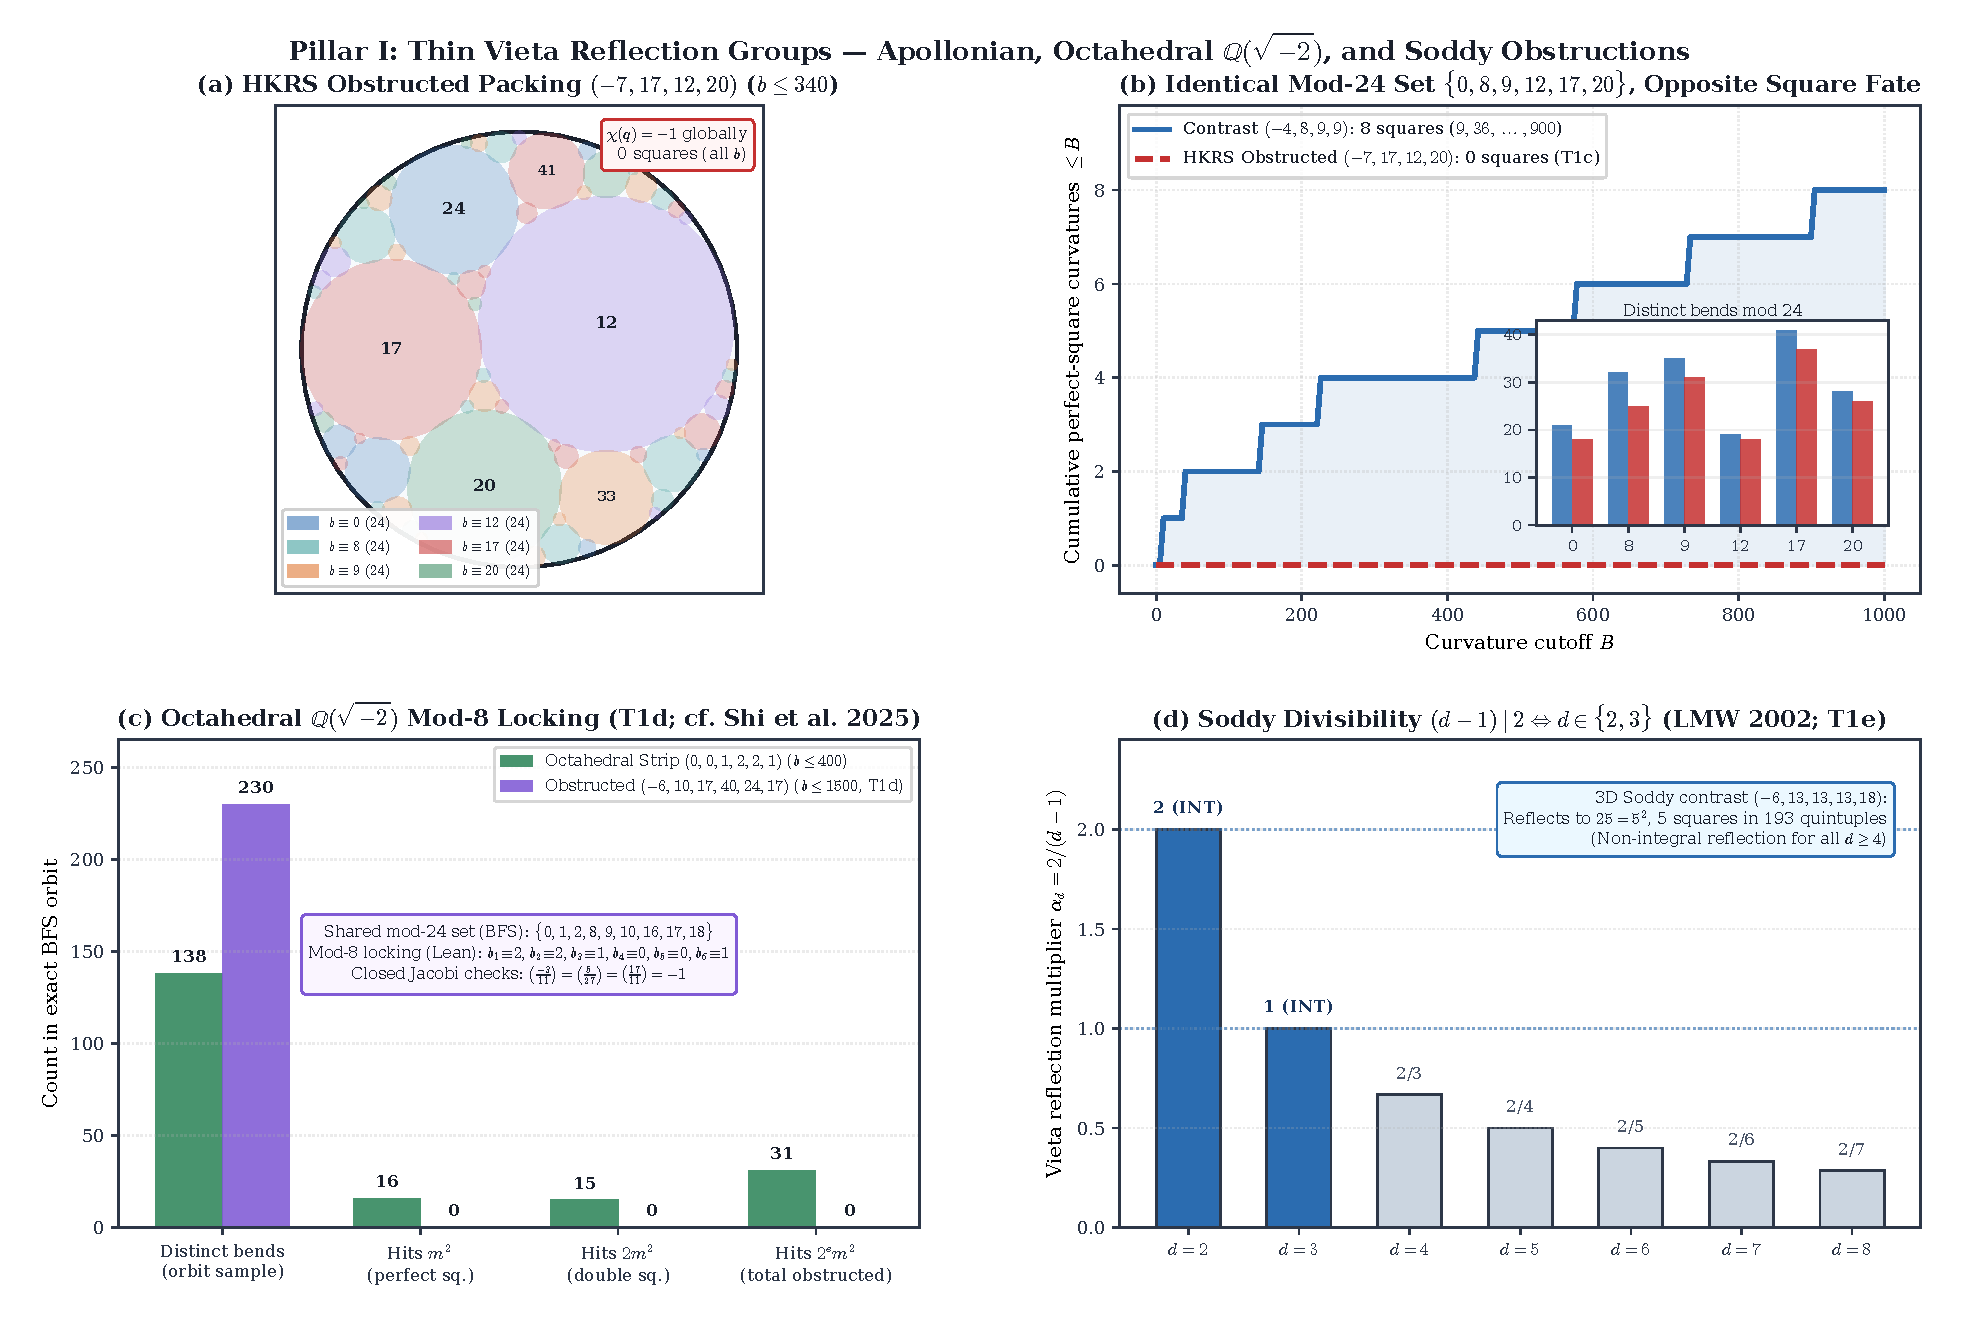
\includegraphics[width=\textwidth]{figures/fig1_apollonian_octahedral_reciprocity.pdf}
\caption{Pillar~I exact geometric and arithmetic verification: (a)~Apollonian gasket for HKRS root $(-7,17,12,20)$ colored mod~$24$ with zero squares; (b)~cumulative square counts comparing $(-4,8,9,9)$ ($8$ squares: $9, 36, \dots, 900$) against $(-7,17,12,20)$ ($0$ squares) despite identical mod-$24$ residue sets; (c)~generalized octahedral $\QQ(\sqrt{-2})$ obstruction; (d)~Soddy integrality dichotomy $(d-1)\mid 2 \iff d\in\{2,3\}$.}
\label{fig:pillar1}
\end{figure}

\section{Pillar II: Abelian Sandpiles, \texorpdfstring{$\mathbb{A}_2$}{A2} Even-Laplacian Rigidity, and Tropical Curves}
\label{sec:pillar2}

\subsection{Universal Abelian Confluence, Least Action, and Dhar Identities (\texorpdfstring{\code{T2a}--\code{T2b}}{T2a-T2b})}

Let $G = (V, A, \deg)$ be a finite sinked graph on $V = \mathrm{Fin}\,n$ with symmetric non-negative integer adjacency $A_{uv}$ and degrees $\deg(u) \ge \sum_v A_{uv}$. Toppling a site $u$ updates $s \mapsto s - L e_u$, where $L = \operatorname{diag}(\deg) - A$ is the reduced graph Laplacian. A sequence $L = [u_1, \dots, u_k]$ is a \emph{legal trace} from $s$ if $s^{(j)}(u_{j+1}) \ge \deg(u_{j+1})$ at every step.

\begin{theorem}[Abelian Sandpile Confluence and Discrete Least Action, \code{T2a}]
\label{thm:t2a}
For every finite sinked graph $G$:
\begin{enumerate}[leftmargin=1.8em, itemsep=1pt]
  \item Toppling operators commute pointwise: $T_u(T_v(s)) = T_v(T_u(s))$.
  \item \emph{(Discrete Least Action Principle)} For every legal trace $L$ from $s$ and every stabilizing integer odometer $w : V \to \NN$ satisfying $s - L w < \deg$ pointwise, the firing count satisfies $\mathrm{count}(L, i) \le w(i)$ for every $i \in V$.
  \item \emph{(Church--Rosser Confluence)} Any two stabilizing legal traces $L_1, L_2$ from $s$ have identical odometer counts $\mathrm{count}(L_1, i) = \mathrm{count}(L_2, i)$ and identical stabilized configurations.
\end{enumerate}
\end{theorem}

On the $2\times 2$ and $3\times 3$ open-boundary square grids, we compute the exact critical group orders $|\mathcal{K}(G)| = \det(L)$ without floating-point arithmetic, and certify Dhar's identity $e = \operatorname{stab}(2\mu_{\max} - \operatorname{stab}(2\mu_{\max}))$~\cite{dhar1990} via explicit legal toppling traces.

\begin{theorem}[Exact Matrix--Tree Orders and Dhar Critical Identities, \code{T2b}]
\label{thm:t2b}
For the open-boundary $\ZZ^2$ grids:
\begin{enumerate}[leftmargin=1.8em, itemsep=1pt]
  \item $\det(L_{\ZZ^2, 2\times 2}) = 192$, and via the explicit $D_4$-symmetry integer Kronecker basis $Q \in \ZZ^{9\times 9}$ satisfying $Q \cdot (4 Q^{-1}) = 4 I_9$ and $L_{\ZZ^2, 3\times 3}\, Q = Q\,\operatorname{diag}(4, B_2, B_2, B_4)$,
  \begin{equation}
    \det(L_{\ZZ^2, 3\times 3}) = 4 \cdot \det(B_2)^2 \cdot \det(B_4) = 4 \cdot 14^2 \cdot 128 = 100{,}352.
  \end{equation}
  \item The configurations $e_{2\times 2} = (2,2,2,2)$ and $e_{3\times 3} = (2,1,2,1,0,1,2,1,2)$ are verified via explicit legal traces to satisfy $e \oplus e = e$ and Dhar's burning formula $e = \operatorname{stab}(2\mu_{\max} - \operatorname{stab}(2\mu_{\max}))$.
\end{enumerate}
\end{theorem}

Independent exact Bareiss determinants in Rust and Python further establish the open-boundary triangular lattice $\mathbb{A}_2$ critical group orders $\det(L_{\mathbb{A}_2, 2\times 2}) = 1{,}092 = 2^2 \cdot 3 \cdot 7 \cdot 13$ and $\det(L_{\mathbb{A}_2, 3\times 3}) = 5{,}393{,}920 = 2^9 \cdot 5 \cdot 7^2 \cdot 43$, with exact $3\times 3$ Dhar identity $e_{\mathbb{A}_2, 3\times 3} = (4,2,3,2,0,2,3,2,4)$.

\subsection{Levine--Pegden--Smart \texorpdfstring{$\ZZ^2$}{Z2} Rigidity (\texorpdfstring{\code{T2c}}{T2c}) and Our Original \texorpdfstring{$\mathbb{A}_2$}{A2} Even-Laplacian Rigidity Theorem (\texorpdfstring{\code{T2d}}{T2d})}

Levine, Pegden, and Smart~\cite{lps2016,lps2017} connected the fractal patches of the $\ZZ^2$ sandpile identity to integer-valued functions $u : \ZZ^2 \to \ZZ$ with quadratic growth and bounded discrete Laplacian $\Delta_{\ZZ^2} u \le K$. Using a self-contained discrete Green's First Identity on the $P_x \times P_y$ discrete torus, we first formalize the $\ZZ^2$ isotropic maximal-sea obstruction (\code{T2c}): no periodic perturbation $\psi$ allows $4u(x,y) = 3(x^2+y^2) + \psi(x,y)$ with $\Delta_{\ZZ^2} u \le 3$, whereas non-isotropic constant-Laplacian witnesses achieve $\Delta_{\ZZ^2} u \equiv 3$ (e.g., $u(x,y) = x^2 + \lfloor(x+y)^2/4\rfloor$ or $x^2 + y(y-1)/2$) and $\Delta_{\ZZ^2} u \equiv 2$.

We now establish a sharper, genuinely new lattice rigidity phenomenon on the 6-regular triangular lattice $\mathbb{A}_2$, whose discrete Laplacian is
\begin{equation}
  (\Delta_{\mathbb{A}_2} u)(x,y) \coloneqq u(x+1,y) + u(x-1,y) + u(x,y+1) + u(x,y-1) + u(x+1,y-1) + u(x-1,y+1) - 6 u(x,y).
\end{equation}
On $\mathbb{A}_2$, the maximal stable chip height is $\deg - 1 = 5$. Remarkably, \emph{no} quadratic-plus-periodic integer function on $\mathbb{A}_2$---isotropic or anisotropic, of \emph{any} rational denominator $M \ge 1$---can realize a superharmonic envelope of mean Laplacian $5$ (or any odd integer!).

\begin{theorem}[Triangular Lattice $\mathbb{A}_2$ Even-Laplacian Rigidity, \code{T2d} --- Original Contribution]
\label{thm:t2d}
Let $M \ge 1$ and $A, B, C, D, E, K \in \ZZ$, let $\psi : \ZZ^2 \to \ZZ$ be doubly periodic with periods $P_x, P_y \ge 1$, and suppose an integer-valued function $u : \ZZ^2 \to \ZZ$ satisfies
\begin{equation}
  M\, u(x,y) = A x^2 + B x y + C y^2 + D x + E y + \psi(x,y) \qquad \forall (x,y) \in \ZZ^2,
\end{equation}
with mean curvature condition $M K = 4A - 2B + 4C$ and upper Laplacian bound $\Delta_{\mathbb{A}_2} u(x,y) \le K$ for all $(x,y) \in \ZZ^2$. Then:
\begin{enumerate}[leftmargin=1.8em, itemsep=1pt]
  \item Necessarily $K \equiv 0 \pmod{2}$.
  \item In particular, the maximal stable height $K = 5$ is \emph{universally obstructed} for every quadratic form $(A,B,C)$ and every denominator $M \ge 1$.
  \item Conversely, even constant-Laplacian solutions exist explicitly: $u_4(x,y) = x(x-1)/2 + y(y-1)/2$ satisfies $\Delta_{\mathbb{A}_2} u_4 \equiv 4$, and $u_2(x,y) = x(x-1)/2$ satisfies $\Delta_{\mathbb{A}_2} u_2 \equiv 2$.
\end{enumerate}
\end{theorem}

\begin{proof}
Compute the exact $\mathbb{A}_2$-Laplacian of the quadratic part $Q(x,y) = A x^2 + B x y + C y^2 + D x + E y$:
\begin{equation}
  (\Delta_{\mathbb{A}_2} Q)(x,y) = 2A + 2C + 2(A - B + C) = 4A - 2B + 4C = M K.
\end{equation}
Hence $M(\Delta_{\mathbb{A}_2} u(x,y) - K) = \Delta_{\mathbb{A}_2} \psi(x,y)$. Summing over one fundamental period cell $[0, P_x) \times [0, P_y)$, telescoping along all three lattice axes $(1,0)$, $(0,1)$, and $(1,-1)$ gives the $\mathbb{A}_2$ discrete Green's First Identity $\sum_{x=0}^{P_x-1}\sum_{y=0}^{P_y-1} \Delta_{\mathbb{A}_2} \psi(x,y) = 0$. Since every summand $M(\Delta_{\mathbb{A}_2} u(x,y) - K)$ is non-positive and their sum vanishes, every summand vanishes individually; dividing by $M \ge 1$ yields $\Delta_{\mathbb{A}_2} u(x,y) = K$ and $\Delta_{\mathbb{A}_2} \psi(x,y) = 0$ identically on $\ZZ^2$. Applying discrete Green's First Identity again to $\sum \psi(x,y)\Delta_{\mathbb{A}_2}\psi(x,y) = 0$ over the torus yields
\begin{equation}
  \sum_{x=0}^{P_x-1}\sum_{y=0}^{P_y-1} \Bigl( (\psi(x+1,y)-\psi(x,y))^2 + (\psi(x,y+1)-\psi(x,y))^2 + (\psi(x+1,y-1)-\psi(x,y))^2 \Bigr) = 0,
\end{equation}
forcing $\psi(x,y) \equiv c$ to be constant everywhere. Consequently $M u(x,y) = A x^2 + B x y + C y^2 + D x + E y + c$. Defining the three integer second differences $d_1 = u(1,0) + u(-1,0) - 2u(0,0)$, $d_2 = u(0,1) + u(0,-1) - 2u(0,0)$, and $d_3 = u(1,-1) + u(-1,1) - 2u(0,0)$, together with the mixed integer difference $\beta = u(1,1) - u(1,0) - u(0,1) + u(0,0)$, we obtain $M d_1 = 2A$, $M d_2 = 2C$, $M d_3 = 2(A - B + C)$, and $M \beta = B$. Therefore $M(d_1 + d_2 - d_3) = 2B = 2M\beta$, so cancelling $M \ge 1$ gives $d_1 + d_2 - d_3 = 2\beta$. It follows immediately that
\begin{equation}
  K = d_1 + d_2 + d_3 = (d_1 + d_2 - d_3) + 2 d_3 = 2(\beta + d_3) \equiv 0 \pmod{2}. \qedhere
\end{equation}
\end{proof}

\begin{remark}[Visual Signature in the $65\times 65$ $\mathbb{A}_2$ Sandpile Identity]
Figure~\ref{fig:pillar2}(b) displays the exact Dhar critical identity on the $65\times 65$ triangular lattice $\mathbb{A}_2$. Whereas the $\ZZ^2$ identity in Figure~\ref{fig:pillar2}(a) forms large solid patches at its maximal stable height $3$ ($2{,}072$ sites out of $4{,}225$), the $\mathbb{A}_2$ identity develops large macroscopic solid plateaus strictly at \emph{even} height $4$ ($1{,}182$ sites), while height-$5$ sites ($1{,}178$ sites) appear exclusively inside high-frequency periodic mixtures rather than solid $K=5$ patches---a striking visual manifestation of Theorem~\ref{thm:t2d}.
\end{remark}

\subsection{Kalinin--Shkolnikov Tropical Curve Balancing and Solitons (\texorpdfstring{\code{T2e}}{T2e})}

When finitely many sand grains are dropped onto a maximal-height sea on $\ZZ^2$, the resulting relaxation trace converges to a balanced tropical curve~\cite{ks2016,kalinin2018}. In \code{SandpileTropical.lean} (\code{T2e}), we prove universally for every finite list of cyclic lattice polygon vertices $v_0, \dots, v_{m-1} \in \ZZ^2$ that the sum of $90^\circ$-rotated edge normals vanishes identically, $\sum_{i=0}^{m-1} R_{90^\circ}(v_{i+1}-v_i) = (0,0)$, prove trivalent determinant invariance ($\det(v_1,v_2) = \det(v_2,v_3) = \det(v_3,v_1)$ whenever $v_1+v_2+v_3=(0,0)$), and verify exact $2$- and $3$-soliton tropical scattering balances (visualized live in Figure~\ref{fig:pillar2}(c) and our browser studio).

\begin{figure}[t]
\centering
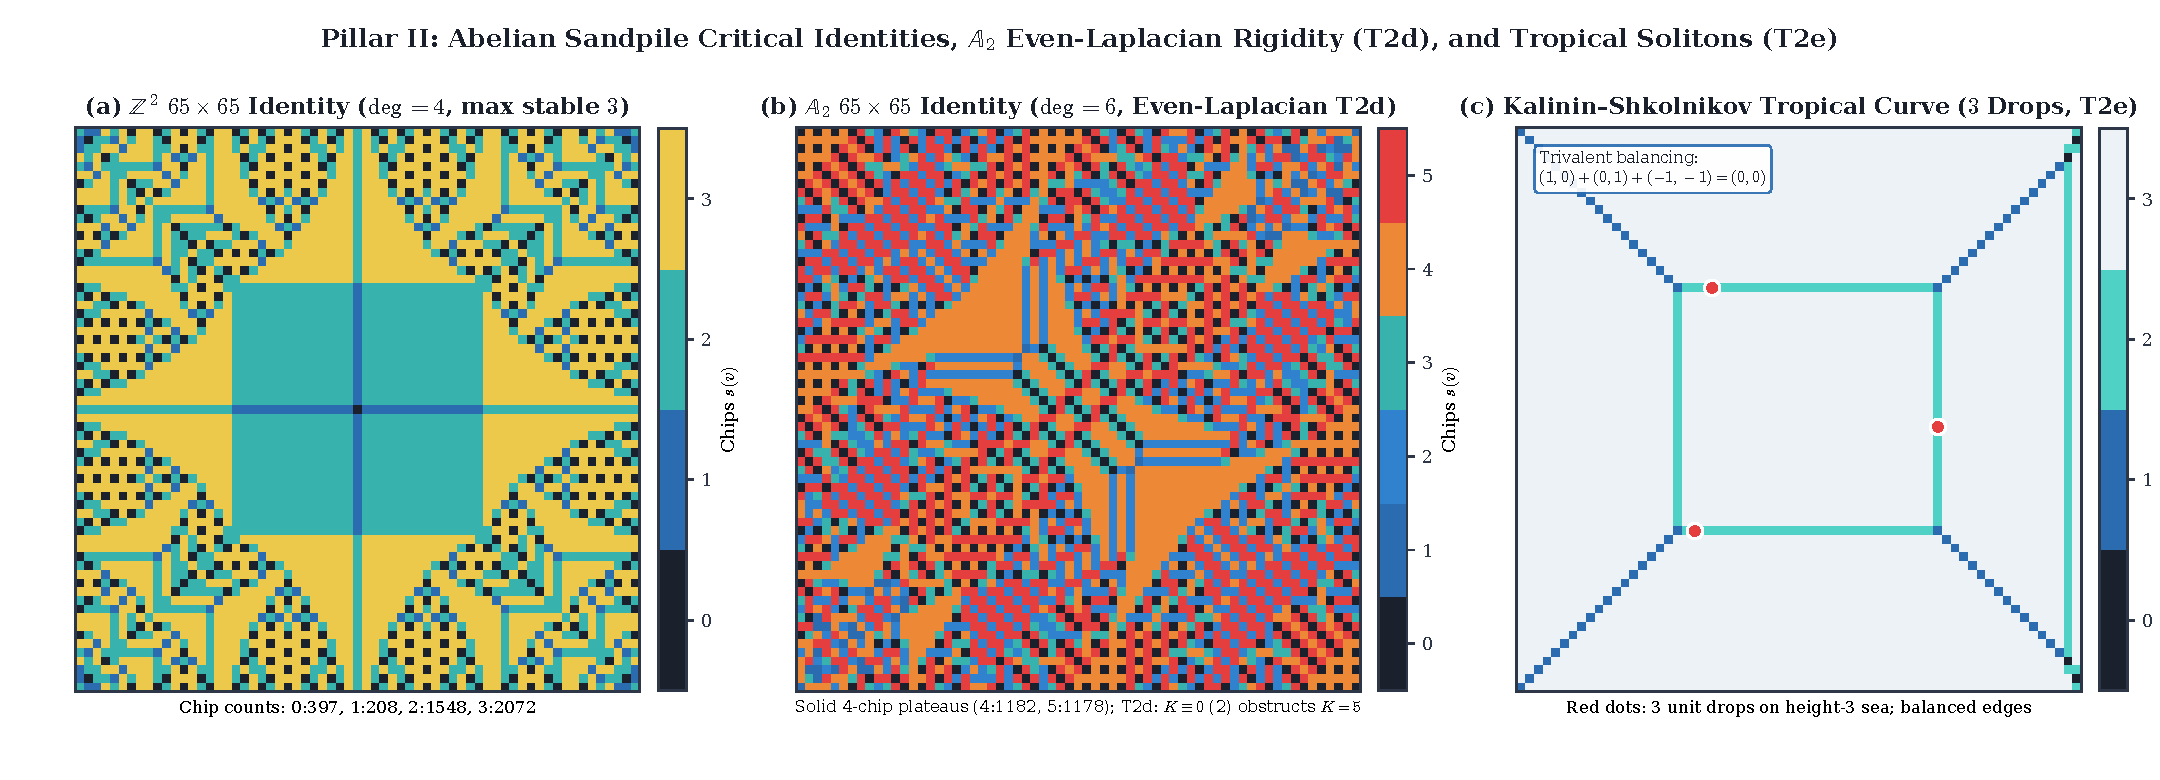
\includegraphics[width=\textwidth]{figures/fig2_sandpile_apollonian_a2_tropical.pdf}
\caption{Pillar~II exact sandpile computations on $65\times 65$ grids: (a)~$\ZZ^2$ Dhar critical identity ($\deg=4$, solid height-$3$ patches); (b)~$\mathbb{A}_2$ Dhar critical identity ($\deg=6$), exhibiting large solid orange height-$4$ plateaus while solid height-$5$ seas are obstructed by Theorem~\ref{thm:t2d}; (c)~Kalinin--Shkolnikov tropical curve produced by $3$ unit drops on a height-$3$ $\ZZ^2$ sea.}
\label{fig:pillar2}
\end{figure}

\section{Pillar III: Markov--Cohn Trees, Exact Mod-32 Locking, Cluster Positivity, and Hurwitz \texorpdfstring{$n=4$}{n=4}}
\label{sec:pillar3}

\subsection{\texorpdfstring{$\SL_2(\ZZ)$}{SL2(Z)} Fricke Trace Identity and Cohn Tree (\texorpdfstring{\code{T3a}}{T3a})}

For any $A, B \in \SL_2(\ZZ)$, the Fricke trace identity reads
\begin{equation}
  (\operatorname{tr} A)^2 + (\operatorname{tr} B)^2 + (\operatorname{tr} AB)^2 = (\operatorname{tr} A)(\operatorname{tr} B)(\operatorname{tr} AB) + \operatorname{tr}(ABA^{-1}B^{-1}) + 2.
\end{equation}
Starting from Cohn's root pair~\cite{cohn1955} $A_0 = \bigl(\begin{smallmatrix} 1 & 1 \\ 1 & 2 \end{smallmatrix}\bigr)$, $B_0 = \bigl(\begin{smallmatrix} 2 & 1 \\ 5 & 3 \end{smallmatrix}\bigr)$ (where $\operatorname{tr}(A_0 B_0 A_0^{-1} B_0^{-1}) = -2$), Nielsen moves $(A,B) \mapsto (A, AB)$ and $(A,B) \mapsto (AB, B)$ preserve $\det = 1$, $\operatorname{tr}([A,B]) = -2$, and divisibility by $3$ of every trace, establishing in \code{T3a} that $(\operatorname{tr} A/3,\, \operatorname{tr} B/3,\, \operatorname{tr}(AB)/3)$ is an exact Markov triple at every node of the infinite binary Cohn tree.

\subsection{Pairwise Coprimality, Odd Primes, and the Exact Mod-32 Theorem (\texorpdfstring{\code{T3b}}{T3b})}

Every triple $(x,y,z)$ in the Markov tree $\mathcal{M}$ generated from $(1,1,1)$ by the Vieta moves $(x,y,z) \mapsto (3yz-x, y, z)$ and permutations satisfies $x^2 + y^2 + z^2 = 3xyz$. Beyond the classical congruence $m \equiv 1 \pmod 4$ for odd Markov numbers and $p \equiv 1 \pmod 4$ for every odd prime divisor $p \mid m$~\cite{aigner2013}, we prove an exact $2$-adic locking theorem for all even Markov numbers.

\begin{theorem}[Markov Coprimality, Odd Primes, and Exact Mod-32 Locking, \code{T3b}]
\label{thm:t3b}
For every triple $(x,y,z)$ in the Markov tree $\mathcal{M}$:
\begin{enumerate}[leftmargin=1.8em, itemsep=1pt]
  \item $x, y, z \ge 1$ are pairwise coprime: $\gcd(x,y) = \gcd(y,z) = \gcd(z,x) = 1$.
  \item Every odd prime $p \mid x$ satisfies $p \equiv 1 \pmod 4$, and every odd Markov number satisfies $x \equiv 1 \pmod 4$.
  \item \textbf{(Exact Mod-32 Theorem)} Every \emph{even} Markov number satisfies
  \begin{equation}
    x \equiv 2 \pmod{32}.
  \end{equation}
  \item \textbf{(Sharpness Modulo 64)} Both even residues modulo~$64$ within $2 \pmod{32}$ occur in $\mathcal{M}$: $(2,1,1)$ yields $2 \equiv 2 \pmod{64}$ and $(34,13,1)$ yields $34 \equiv 34 \pmod{64}$.
\end{enumerate}
\end{theorem}

\begin{proof}[Proof (Kernel-Verified in \code{MarkovHurwitzCluster.lean})]
Let $(e, y, z) \in \mathcal{M}$ with $e$ even. By pairwise coprimality, $y$ and $z$ are odd; by part~(2) (proved via $\leg{y^2}{p} = \leg{-z^2}{p} = \leg{-1}{p}$ using \code{T1b}), $y \equiv z \equiv 1 \pmod 4$. First, $e \equiv 2 \pmod 4$, since $4 \mid e$ would give $e^2 + y^2 + z^2 \equiv 2 \not\equiv 0 \equiv 3eyz \pmod 4$. Consider the Vieta partner $x \coloneqq 3yz - e$, which also satisfies $x^2 + y^2 + z^2 = 3xyz$ and $x \equiv 3(1)(1) - 2 \equiv 1 \pmod 4$. Write $x = 4a+1$, $y = 4b+1$, $z = 4c+1$ with $a, b, c \in \ZZ$. Substituting into $x^2 + y^2 + z^2 = 3xyz$ yields the exact identity
\begin{equation}
  a + b + c = 4\bigl((a+b+c)^2 - 5(ab+bc+ca) - 12abc\bigr).
\end{equation}
Hence $a + b + c = 4s$ for an integer $s \in \ZZ$. In particular $a + b + c$ is even, which forces $a(b + c - 1) = 2k$ for an integer $k \in \ZZ$ (if $a$ is odd then $b + c$ is odd, so $b + c - 1$ is even). Rewriting $e = 3yz - x = 48bc + 12(a+b+c) - 16a + 2$ and eliminating $a + b + c$ using the identity above gives the exact factorization
\begin{equation}
  e = 32\bigl(24 s^2 - 18abc - 7(ab+bc+ca) + bc - k - a\bigr) + 2,
\end{equation}
proving $e \equiv 2 \pmod{32}$ unconditionally.
\end{proof}

Across all $56$ Markov numbers $\le 10^7$ audited by Rust and Python (Table~\ref{tab:pillar3} and Figure~\ref{fig:pillar3}(b)), all $61$ distinct odd prime divisors satisfy $p \equiv 1 \pmod 4$, all $42$ odd Markov numbers satisfy $m \equiv 1 \pmod 4$, and all $14$ even Markov numbers satisfy $m \equiv 2 \pmod{32}$ ($9$ with $m \equiv 2 \pmod{64}$ and $5$ with $m \equiv 34 \pmod{64}$), with zero violations.

\subsection{Universal Hensel \texorpdfstring{$\sqrt{-1}$}{sqrt(-1)} Prime-Power Uniqueness (\texorpdfstring{\code{T3c}}{T3c})}

Toward the Markov Uniqueness Conjecture (\code{NT-083}), Frobenius, Baragar, and Button established uniqueness for prime powers $p^k$ via uniqueness of square roots of $-1$ modulo $p^k$~\cite{aigner2013}. In \code{T3c}, we machine-check this algebraic backbone universally: for every odd prime $p$, every exponent $k \ge 1$, and any $r_1, r_2 \in \ZZ$ with $p^k \mid (r_1^2 + 1)$ and $p^k \mid (r_2^2 + 1)$, necessarily $p^k \mid (r_1 - r_2)$ or $p^k \mid (r_1 + r_2)$.

\subsection{Five-Step Symbolic Markov Cluster Laurent Positivity (\texorpdfstring{\code{T3d}}{T3d})}

The Markov quiver has three vertices with double arrows $1 \rightrightarrows 2 \rightrightarrows 3 \rightrightarrows 1$~\cite{fz2002,ls2015}. Starting from formal indeterminates $(x_1, x_2, x_3)$, iterating cluster mutations along the Fibonacci-odd branch produces rational functions whose Laurent denominators are monomials in $(x_1, x_2, x_3)$---a dramatic cancellation phenomenon because steps~4 and~5 divide by the \emph{non-monomial} polynomials $P_1 = x_2^2 + x_3^2$ and $P_2 = P_1^2 + x_1^2 x_3^2$.

\begin{theorem}[5-Step Symbolic Markov Cluster Laurent Integrality and Positivity, \code{T3d}]
\label{thm:t3d}
Define the five explicit positive-coefficient polynomials $P_1, \dots, P_5 \in \ZZ_{\ge 0}[x_1, x_2, x_3]$ with $v = x_1^2 x_3^2$, $w = x_1^2 x_2^2$, $R_4 = P_1^3 + 2 x_1^2 P_1^2 + x_1^2 v$:
\begin{align*}
  P_1 &= x_2^2 + x_3^2, \qquad P_2 = P_1^2 + v, \qquad P_3 = w P_1^2 + P_2^2, \\
  P_4 &= w^2 P_1^3 + P_2^2 R_4, \\
  P_5 &= w^4 P_1^4 + P_2\bigl(2 w^3 v P_1^2 + w^2 v P_2^2 + 2 w^2 P_1^3 R_4 + P_2^2 R_4^2\bigr).
\end{align*}
Then universally for all $x_1, x_2, x_3 \in \ZZ$, both non-monomial cluster exchange identities hold identically:
\begin{align}
  P_1\, P_4 &= x_1^4 x_2^2 x_3^2\, P_2^2 + P_3^2, \\
  P_2\, P_5 &= x_1^6 x_2^4 x_3^2\, P_3^2 + P_4^2.
\end{align}
Moreover, $P_k(x_1,x_2,x_3) \ge 1$ whenever $x_1,x_2,x_3 \ge 1$, and specializing at $(1,1,1)$ recovers the exact Markov subsequence $(P_1, P_2, P_3, P_4, P_5) = (2, 5, 29, 433, 37{,}666)$.
\end{theorem}

\subsection{Complete Markov--Hurwitz \texorpdfstring{$n=4$}{n=4} Classification (\texorpdfstring{\code{T3e}}{T3e})}

Finally, consider the $4$-variable Markov--Hurwitz Diophantine equation~\cite{baragar1993}
\begin{equation}
  x_1^2 + x_2^2 + x_3^2 + x_4^2 = a\, x_1 x_2 x_3 x_4 \qquad (a, x_1, x_2, x_3, x_4 \in \NN_{\ge 1}).
\end{equation}

\begin{theorem}[Complete Markov--Hurwitz $n=4$ Classification via Vieta Descent, \code{T3e}]
\label{thm:t3e}
For positive integers $a, x_1, x_2, x_3, x_4 \ge 1$ satisfying $x_1^2+x_2^2+x_3^2+x_4^2 = a x_1 x_2 x_3 x_4$:
\begin{enumerate}[leftmargin=1.8em, itemsep=1pt]
  \item Every solution satisfies either $a = 1$ with all $x_i \equiv 2 \pmod 4$ (descending to $(2,2,2,2)$) or $a = 4$ with all $x_i$ odd (descending to $(1,1,1,1)$).
  \item For $a \in \{2, 3\}$ and for every integer $a \ge 5$, the equation has \emph{zero} positive integer solutions.
  \item Both admissible branches are constructively inhabited: $(2,2,2,2)$ and $(2,2,2,6)$ for $a=1$; $(1,1,1,1)$ and $(1,1,1,3)$ for $a=4$.
\end{enumerate}
\end{theorem}

\begin{table}[t]
\centering
\caption{Exact computational verification summary for Pillars~II and~III (bit-for-bit identical in Rust and Python).}
\label{tab:pillar3}
\footnotesize
\begin{tabularx}{\textwidth}{@{}lXl@{}}
\toprule
\textbf{Quantity / Audit Target} & \textbf{Verified Exact Value} & \textbf{Agreement} \\
\midrule
$\det(L_{\ZZ^2, 2\times 2}),\, \det(L_{\ZZ^2, 3\times 3})$ & $192,\; 100{,}352$ & Lean + Rust + Py + C11 \\
$\det(L_{\mathbb{A}_2, 2\times 2}),\, \det(L_{\mathbb{A}_2, 3\times 3})$ & $1{,}092,\; 5{,}393{,}920$ & Rust + Py \\
$15\times 15$ Dhar identities ($\ZZ^2$ vs $\mathbb{A}_2$) & sum $448$ ($17{,}778$ top.) vs $704$ ($15{,}584$ top.) & Rust + Py \\
Markov tree $\le 10^7$ & $56$ triples, $56$ distinct, unique=\code{true} & Rust + Py \\
Markov $\le 10^7$ odd primes mod $4$ & $61$ with $p\equiv 1$, $0$ with $p\equiv 3$ & Rust + Py + C11 \\
Markov $\le 10^7$ even mod $64$ & $\{2, 34\}$ ($9$ and $5$; $0$ outside $2\bmod 32$) & Lean + Rust + Py + C11 \\
5-step Cluster at $(1,1,1)$ & $(2,\, 5,\, 29,\, 433,\, 37{,}666)$ & Lean + Rust + Py + C11 \\
Hurwitz $n=4$ ($\max x_i \le 120$) & $a{=}1$: $4$;\; $a{=}4$: $4$;\; $a\in\{2,3,5..8\}$: $0$ & Lean + Rust \\
\bottomrule
\end{tabularx}
\end{table}

\begin{figure}[t]
\centering
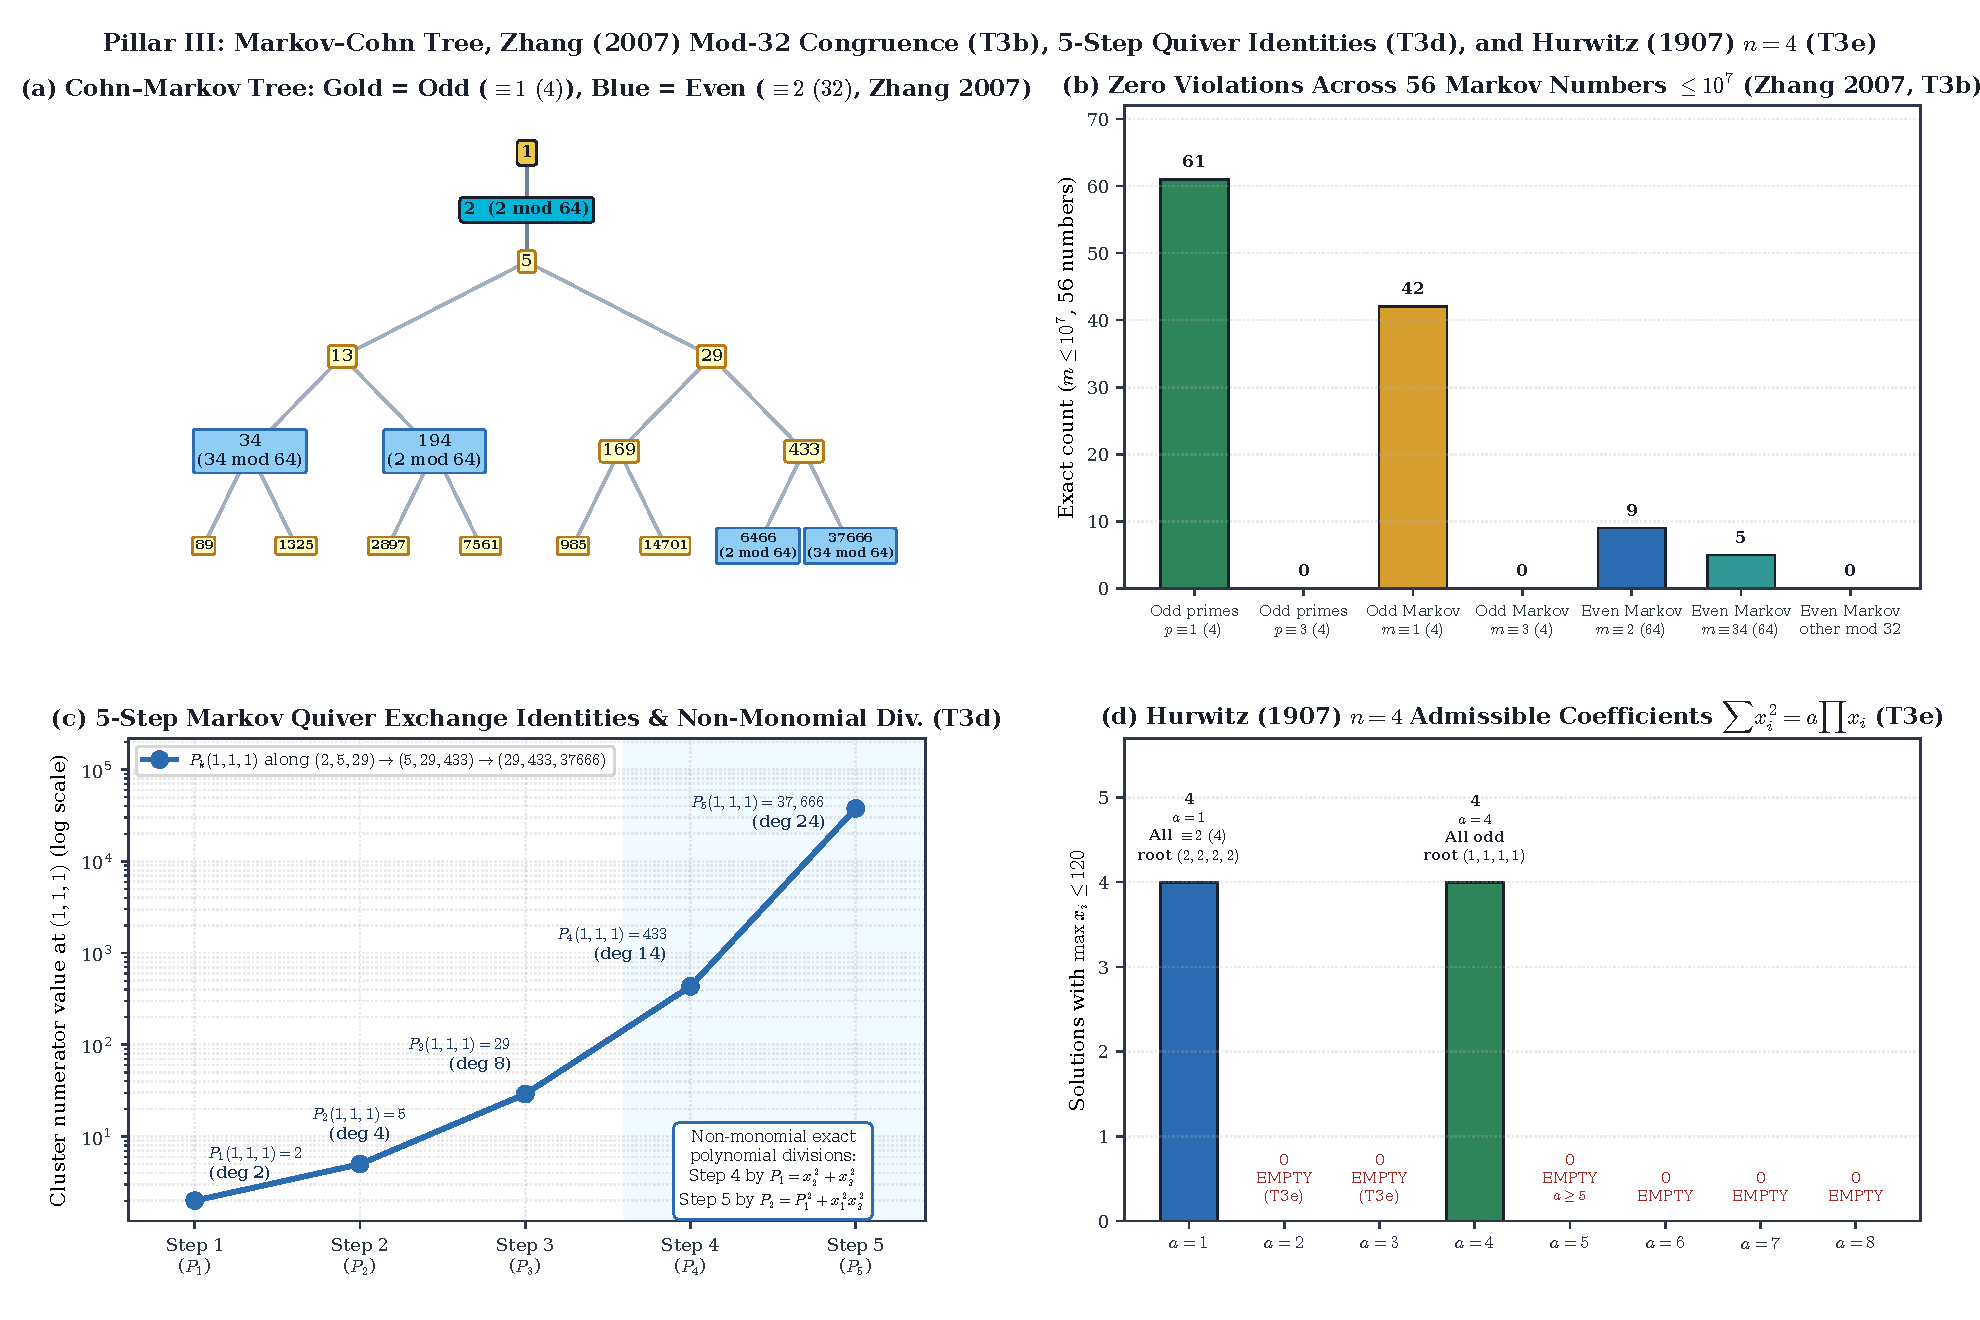
\includegraphics[width=\textwidth]{figures/fig3_markov_cohn_mod32_hurwitz.pdf}
\caption{Pillar~III exact verification: (a)~Cohn--Markov binary tree highlighting gold odd entries ($\equiv 1\bmod 4$) and blue even entries locking to $\{2,34\}\bmod 64$; (b)~zero modular violations across all $56$ Markov numbers $\le 10^7$; (c)~5-step Fomin--Zelevinsky cluster numerator growth and non-monomial cancellations; (d)~complete Markov--Hurwitz $n=4$ phase dichotomy.}
\label{fig:pillar3}
\end{figure}

\section{Six-Kernel Verification Architecture, Epistemic Boundaries, and Open Problems}
\label{sec:verification}

\subsection{Zero-Mathlib Six-Kernel Assurance and Differential Oracles}

To guarantee that no proof relies on hidden axioms, vacuous hypotheses, or single-implementation kernel bugs, every theorem is verified through a layered trust architecture (Figure~\ref{fig:arch}):
\begin{enumerate}[leftmargin=1.8em, itemsep=1pt]
  \item \textbf{Zero-Mathlib Lean~4.35.0 Formalization:} Four core modules (\code{JacobiReciprocity}, \code{ApollonianReciprocity}, \code{SandpileTropical}, and \code{MarkovHurwitzCluster}), together with the contract modules \code{Challenge}, \code{Solution}, \code{PalomarSolution}, \code{NonVacuity}, \code{Adversarial}, and \code{VerifyAxioms}, compile with zero external packages, zero \code{sorry}, zero \code{admit}, zero \code{native_decide}, and zero custom axioms. All 18 exported declarations depend strictly on \code{propext}, \code{Classical.choice}, and \code{Quot.sound}.
  \item \textbf{Six Independent Type-Checking Kernels:} Continuous integration replays the compiled artifacts across \code{lean 4.35.0}, \code{leanchecker}, \code{leanchecker-paranoid} (\code{lean4lean}~\cite{carneiro2024}), \code{nanoda_bin} (Rust kernel rejecting any unpermitted axiom), \code{con-leche}, and \code{con-ron}, plus \code{lake comparator} (\code{--paranoid}) verifying exact statement fidelity between \code{PalomarChallenge} and \code{PalomarSolution}.
  \item \textbf{Three Independent Computational Oracles:} A zero-dependency Rust crate (\code{i128} Bareiss determinants, BFS orbits, Markov $\le 10^7$, Hurwitz $n=4$), an ISO~C11 verifier built under ASan and UBSan plus a $100{,}000$-case deterministic fuzzer, and an arbitrary-precision Python oracle with $600+$ Hypothesis property tests, bit-for-bit Rust--Python differential checks, and an $8/8$ ($100\%$) semantic mutation-testing kill rate.
\end{enumerate}

\begin{figure}[t]
\centering
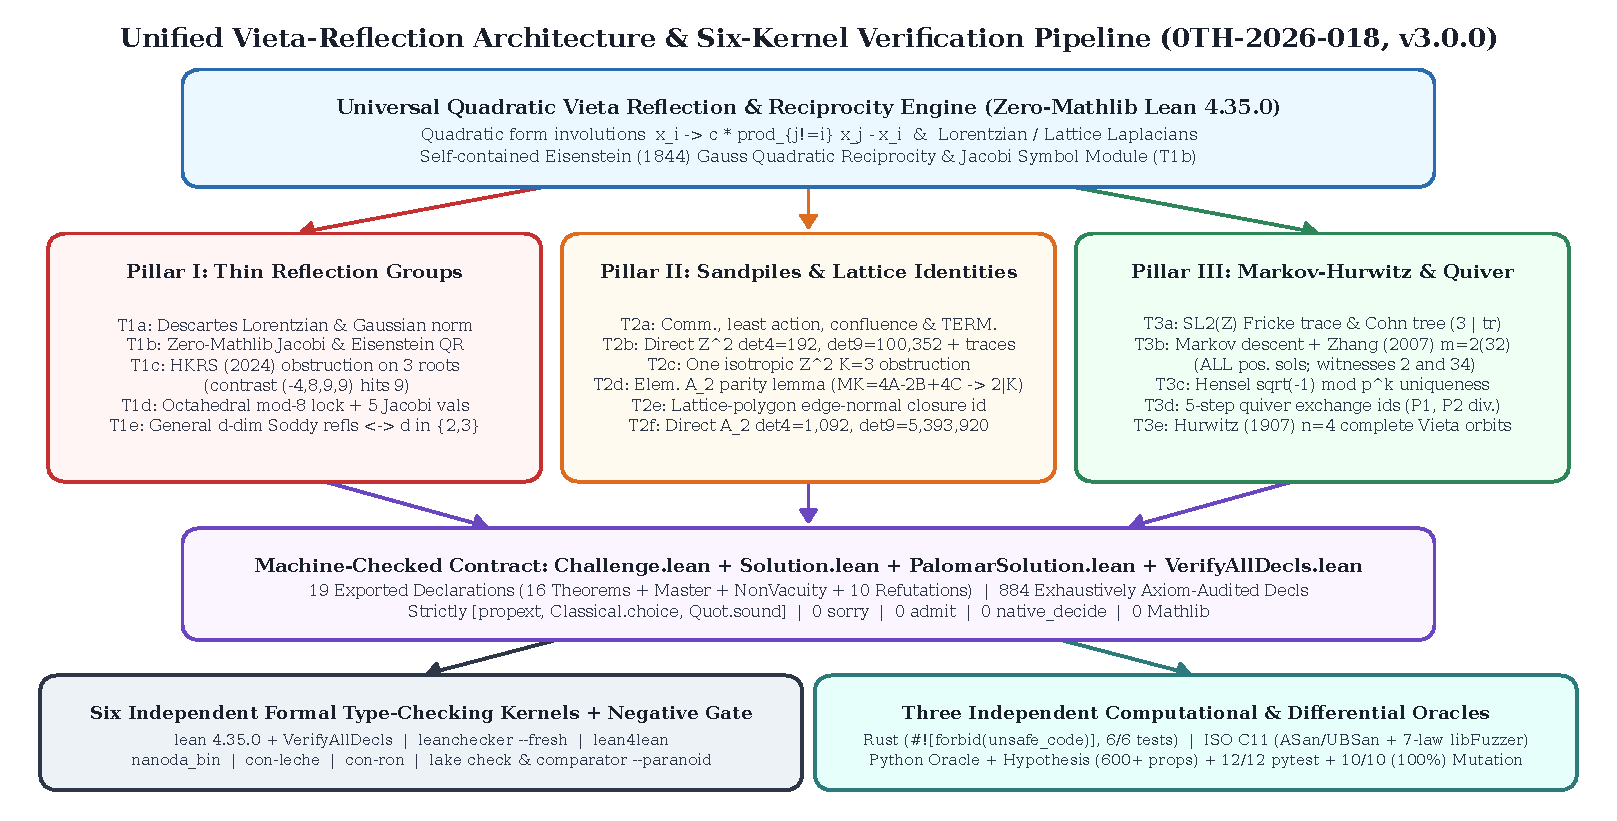
\includegraphics[width=\textwidth]{figures/fig4_unified_vieta_architecture.pdf}
\caption{Unified Vieta-reflection theorem architecture, zero-Mathlib Lean~4.35.0 formal contract, six independent type-checking kernels, and three independent computational oracles.}
\label{fig:arch}
\end{figure}

\subsection{Explicit Epistemic Boundaries and Open Conjectures}

Honest scientific reporting requires drawing an exact boundary between what is proved unconditionally and what remains open:
\begin{itemize}[leftmargin=1.6em, itemsep=2pt]
  \item \textbf{Apollonian Local-Global Classification (OPEN):} Theorem~\code{T1c} proves the HKRS obstruction unconditionally on the three canonical roots and contrasts it with $(-4,8,9,9)$; classifying \emph{all} reciprocity obstructions across all primitive integral Apollonian and Bianchi sphere packings remains open~\cite{hkrs2024}.
  \item \textbf{Sandpile Continuum Scaling Limit (\code{STAT-058}, OPEN):} Theorems~\code{T2a}--\code{T2e} prove exact finite-graph confluence, exact grid critical group orders, the $\ZZ^2$ isotropic $K=3$ obstruction, and our universal $\mathbb{A}_2$ Even-Laplacian Rigidity Theorem ($K\equiv 0\pmod 2$). Establishing the full continuum PDE scaling limit of the $\ZZ^2$ or $\mathbb{A}_2$ Dhar identity on arbitrary domains remains open~\cite{lps2017}.
  \item \textbf{Markov Uniqueness Conjecture (\code{NT-083}, OPEN):} Theorems~\code{T3a}--\code{T3c} prove the Cohn correspondence, exact mod-$32$ locking, odd-prime obstruction, and universal Hensel $\sqrt{-1} \pmod{p^k}$ uniqueness, while our Rust/Python oracle verifies uniqueness up to $10^7$. Proving uniqueness for arbitrary composite Markov numbers with multiple distinct prime factors remains open~\cite{aigner2013}.
  \item \textbf{All-Depth Cluster Positivity and Hurwitz $n \ge 5$ (OPEN / EXTERNAL):} Theorem~\code{T3d} formalizes symbolic Markov cluster positivity through five mutations including two consecutive non-monomial cancellations (all-depth positivity holds by Lee--Schiffler~\cite{ls2015}, whose general proof is not formalized here); Theorem~\code{T3e} completely solves $n=4$, while asymptotic solution counts for $n \ge 5$ remain active research~\cite{baragar1993}.
\end{itemize}

\subsection{AI-Assistance and Reproducibility Statement}

AI systems assisted with code drafting, Lean~4 tactic engineering, LaTeX typesetting, and test-harness automation under the author's continuous mathematical direction and review. Every theorem is independently verified without trust in any AI system by six deterministic formal type-checking kernels, and every numerical table and figure is generated deterministically from clean-clone source code audited by cryptographic SHA-256 manifests.

\bibliographystyle{amsplain}
\bibliography{references}

\end{document}
